%Custom Functions
\newcommand{\CompanyName}{TT} % update later

\documentclass[conference]{IEEEtran}
\IEEEoverridecommandlockouts
% The preceding line is only needed to identify funding in the first footnote. If that is unneeded, please comment it out.
%\usepackage{cite}
\usepackage{amsmath,amssymb,amsfonts}
\usepackage{algorithmic}
\usepackage{graphicx}
\usepackage{textcomp}
\usepackage{xcolor}

\usepackage{pdflscape}

\usepackage[utf8]{inputenc}
\usepackage{fancyhdr}
\usepackage{lastpage}

% Please add the following required packages to your document preamble:
\usepackage{multirow}
\usepackage[numbers]{natbib}

\usepackage{listings}
\usepackage{hyperref}
\usepackage{amsmath}

\hypersetup{
    colorlinks=true,
    linkcolor=black,
    filecolor=magenta,      
	urlcolor=cyan
}

\usepackage{listings}
\usepackage{color}

\definecolor{dkgreen}{rgb}{0,0.6,0}
\definecolor{gray}{rgb}{0.5,0.5,0.5}
\definecolor{mauve}{rgb}{0.58,0,0.82}

\lstset{frame=single,
  language=C++,
  showstringspaces=false,
  columns=flexible,
  basicstyle={\small\ttfamily},
  numbers = none,
  numberstyle=\tiny\color{gray},
  keywordstyle=\color{blue},
  commentstyle=\color{dkgreen},
  stringstyle=\color{mauve},
  breaklines=true,
  breakatwhitespace=true,
  tabsize=2
}

\def\BibTeX{{\rm B\kern-.05em{\sc i\kern-.025em b}\kern-.08em
T\kern-.1667em\lower.7ex\hbox{E}\kern-.125emX}}

\fancypagestyle{fancylandscape}{
\fancyhf{} %Clears the header/footer
\fancyfoot{% Footer
\makebox[\textwidth][r]{% Right
  \rlap{\hspace{.75cm}% Push out of margin by \footskip
    \smash{% Remove vertical height
      \raisebox{4.87in}{% Raise vertically
        \rotatebox{90}{Page \thepage\ of \pageref{LastPage}}}}}}}% Rotate counter-clockwise
\renewcommand{\headrulewidth}{0pt}% No header rule
\renewcommand{\footrulewidth}{0pt}% No footer rule
}

\pagestyle{fancyplain}
\fancyhf{}
\fancyfoot[c]{Page \thepage\ of \pageref{LastPage}}
\renewcommand{\headrulewidth}{0pt}

\begin{document}

	\title{VisualPro - Research Proposal}

	\author{\IEEEauthorblockN{1\textsuperscript{st} Given Edward Patch}
	\IEEEauthorblockA{\textit{Software Engineer Student (of BSc Year 3)} \\
    \textit{Independent Project}\\
    \textit{University of Wales Trinity St. Davids (of Mike Dacey)}\\
    Swansea, Wales \\
    Student ID: 1801492}}

     \maketitle
    
    \thispagestyle{plain}
    \pagestyle{plain}
    
    \tableofcontents
	  \vspace{.5cm}

    \begin{abstract}
    \label{abstract}
      This document provides the proposal of the Independent Project. After doing in-depth research and planning, the working title for this project is VisualPro.

      Hypothesis: If visual scripting can write structure and logic of any desired language the user wishes, will this:-
        \begin{itemize}
          \item A: produce a more productive and better work environment.
          \item B: help novices code in any language without knowing different syntax per language.
        \end{itemize}
    \end{abstract}

    \begin{IEEEkeywords}
        Visual Programming, Proposal, Research.
    \end{IEEEkeywords}

    \section{Introduction}
    \label{sec:Introduction}
      VisualPro aims to be a lightweight visual programming pad, which includes the following features:-
      \begin{itemize}
        \item Program in any language with ease.
        \item Enables users to write code in seconds.
        \item A simple Graphical User Interface (GUI) that changes the way Visual Scripting already works.
      \end{itemize}
  
      The prototypes will demonstrate C/C++ libraries working together with a different language, which plays a massive part to archive this task.

      \subsection{Potential growth to VisualPro}
      The dynamics of the custom languages allow new scripting languages. Consequently, it implies but is not limited to, Notebook and Stylus companies benefiting from this product. Take a look at (reference page) for more information on this topic.

      \subsection{Sections}
      The VisualPro Proposal document includes a Literature Review, Aims and Objective, Project Design, Resources and Planning and Reference List.

      The Literature Review section contains segments of academic books and articles related to the project proposal. Within the extensive research, hand-picked books and articles to show what technologies are required to make the idea plausible, narrowing down the project's association towards the Author's study area.
      
      After the Literature Review section, the Aims and Objectives section will give the reader an idea of how the final product will impact society and its user base.
      
      The third section, Project Design, describes the outline of the project process, data collection, risks and limitations and ethical issues. These are essential points that decide if the project breaks any laws or pushes too many boundaries in today's society.
      
      The Resources and Planning section include two sub-sections; Resources Required and Planning Chart. Resources Required sub-section involves Physical Resources \textit{(if any hardware and equipment are required)}, Human Resources \textit{(if any staff are required)} and Other Resources \textit{(if any software or other categories not been mentioned are required)}. The Planning Chart sub-section displays the tasks and time frame within a Gantt Chart, constructed by Microsoft Project~\cite{microsoft_compare_nodate}.

    \section{Literature Review}
    \label{sec:literatureReview}
      \subsection{Productivity and Visual Scripting}
        Multiple books are necessary to capture this question, ``If visual scripting can write structure and logic of any desired language the user wishes, will this produce a more productive and better work environment''. The research also helps understand why visual scripting or interpreted programming languages/scripts are more popular than compiled programming languages and how productivity expands with new access to different tools.

        Productivity, specifically within the software engineering field, Rethinking Productivity in Software Engineering Book states, ``Productivity is a challenging concept to define, describe, and measure for any knowledge work that involves nonroutine creative tasks. Software development is a prime example of knowledge work, as it too often involves poorly defined tasks relying on extensive collaborative and creative endeavors. As in other areas of knowledge work, defining productivity in software development has been a challenge facing both researchers and practitioners who may want to understand and improve it by introducing new tools or processes.'' When reading further into the chapter, the following points evaluate how we should think about productivity:-

        \begin{itemize}
          \item ``Velocity: How fast works gets done.''
          \item ``Quality: How well works gets done.''
          \item ``Satisfaction: How satisfying the work is.''
        \end{itemize}

        After thinking about this, VisualPro, in theory, should increase the rapidity of the individual’s work. Suppose VisualPro changes the way Visual Scripting works today, making it lightweight and understandable compared to existing Visual Scripting (For example, Unreal Engine's Blueprints~\cite{unreal_engine_introduction_nodate}), with the ability to generate any desired code. In that case, the quality and satisfaction of the developer amplify.

        To compare the theory to conclude, \textbf{Hypothesis A} and \textbf{B}, page~\pageref{abstract}, two books, Dr. C. Sadowski and Dr. Thomas Zimmerman's~\cite{dr_caitlin_sadowski_rethinking_2019} Book, ``Rethinking Productivity in Software Engineering'', and A. M. Winn and T. J. Smedley’s~\cite{winn_multimedia_1998} Book, ``Multimedia Workshop: Exploring the Benefits of a Visual Scripting Language'', helps decide the decision.

        \begin{center}
           A: produce a more productive and better work environment.
           B: help novices code in any language without knowing different syntax per language.
        \end{center}
        
        After examining Chapter 1, ``Are Slower Programmers Just More Careful?''~\cite{dr_caitlin_sadowski_rethinking_2019}, figure 1-3 is shown. The dialogue suggested that $O$ symbols represent ``...dynamically typed scripting'' and $\mathbf{X}$ symbols represent ``...statically typed programs'' within the graph. The author was trying to show that script languages might produce productivity, as they require fewer lines of code, but programming languages offer more efficient execution time. In order to complete the analysis of \textbf{Hypothesis A}, it is essential to understand that the proposed idea should act as a script but generate a programming language whilst making an easy-to-use environment. This statement, including the figure shown, with the points mentioned, concludes that \textbf{Hypothesis A} is true if administered accurately.

        A. M. Winn and T. J. Smedley’s~\cite{winn_multimedia_1998} Book, section 3.2, ``The graphical user-interface'',  suggests that Multimedia Workshop (MMW) Visual Scripting is excellent for junior and experienced developers, ``...MMW was carefully designed for easy and natural use...''. The Author’s of this Book mentions that a poor graphical user interface could ``...hinder an assessment of the usefulness of a visual scripting language''. To prove \textbf{Hypothesis B} effective on novices stands true on condition the software is executed correctly and is not complicated or chunky when designing software. This project requires an easy drag and drop method with a simple layout to meet \textbf{Hypothesis B}’s aim.

      \subsection{Markup Languages}
      \label{subsec:lr-markupLanguages}
        \textbf{What is a Markup Language?}\\
        A markup language is essentially a script, which consists of tags and attributes as Erik T. Ray's~\cite{ray_learning_nodate} Book implies in Chapter 2 (Markup and Core Concepts), page 49, ``Just as skeletons give us vertebrates shape and structure, markup does the same for text.'' This quote implies that markup languages offer structures, principally for designs, layouts and arrangement responsibilities. Due to the nature of Markup Languages with the ease of adding tags and attributes, Markup Languages will do the heavy lifting of setting available libraries and syntax for each language.

        \textbf{How will Extensible Markup Language (XML) support custom languages in this project?}\\
          According to G. Costa and R. Ortale~\cite{costa_machine_2018}, Machine learning techniques for XML (co-)clustering by structure and-constrained phrases Book, Chapter 2.1, ``\textit{An \textbf{XML tree} is a rooted, labeled, tree \textbf{t = (V$^{\text{t}}$,r$^{\text{t}}$,E$^{\text{t}}$,$\lambda^{\text{t}}$)} where:}
          \begin{itemize}
            \item \textbf{V$^{\text{t}} \subseteq \mathbb{N}$} is a set of nodes, with \textbf{r$^{\text{t}} \in \text{V}^{\text{t}}$} being the root of \textbf{t};
            \item \textbf{E$^{\text{t}} \subseteq \text{V}^{\text{t}} \times \text{V}^{\text{t}}$} is a set of edges, catching parent-child relationships between nodes of \textbf{t};
            \item \textbf{$\lambda \text{ : V}^{\text{t}} \rightarrow \sum $} is a labelling function, with $\sum$ being the domain of the node tags (or equivalently, labels).''
          \end{itemize}

          The facility of having nodes and attributes means we can expand the XML file with many different syntaxes for different opportunities. If nested nodes are within the parent nodes, then it will increase the performance time of execution. The library that reads through the XML document will only need to select the relevant sub-nodes listed under the parent node instead of reading through every possible node outcome. In theory, users can append languages by reading through the XML document quite efficiently, and the software would read through the XML document without any issues.

    \section{Aims and Objectives}
      \subsection{Aims}
        VisualPro software aims to increase existing software engineers, web developers, and other users in different professions. Productivity would increase and allow individuals to code in many languages without understanding different languages. The software aims to provide custom languages by a markup language with an easy-to-grasp script. Read section~\ref{sec:literatureReview} Literature Review, sub-section~\ref{subsec:lr-markupLanguages}, page~\pageref{subsec:lr-markupLanguages} to understand markup language.
      \subsection{Objectives}
        To achieve the aims mentioned in section~(a reference in aims and objectives), sub-section~(a reference in arms). In order to meet the aims during the production process of the project, the following objectives is a must. These objectives are as follows:-
        \begin{itemize}
          \item Project planning (section:~\ref{sec: resourcesPlanning} Resources and Planning, sub-section:~\ref{subsec:rp-planningChart} Planning Chart, page~\pageref{subsec:rp-planningChart}).
          \item Create prototypes (Existing \href{https://github.com/ShinkuKira21/VisualPro-FinalProject/tree/main/Experience}{programs}~\cite{patch_programming_2021} and \href{https://github.com/ShinkuKira21/VisualPro-FinalProject/tree/main/Libraries}{libraries}~\cite{patch_libraries_2021} to make this possible.).
          \item Conduct surveying, backend unit testing and front-end user interface testing relating to `Program in any language with ease' section~\ref{sec:Introduction}, page~\pageref{sec:Introduction}.
          \item Create a front-end to work with existing libraries, which helps recreate Visual Scripting technology.
          \item Create a backend to communicate with the front-end and generate code based on values the user enters, which should help the user to compose code in seconds.
        \end{itemize}
      
    \section{Project Design}
      \subsection{Outline of Project Process}
        Outline of the project process:-
        \begin{itemize}
          \item Design and produce a front-end to dock the backend libraries.
          \item Convert existing libraries and programs to Dynamic-Link Library (DLL) archives that work with the front-end.
          \item Create a LanguageCompiler (similarly to \href{https://github.com/ShinkuKira21/VisualPro-FinalProject/tree/main/Experience}{Programming Planner}~\cite{patch_programming_2021}) but with custom languages (XML).
          \item Design and create an XML script that tells the backend of what languages are available. The script must be understandable by the user.
          \item Use C \textit{\_declspec(dllexport)}~\cite{microsoft_exporting_2019} to export entry points within the DLL libraries.
        \end{itemize}
        
      \subsection{Data Collection}
        Survey data will not ask for the personal details of the surveyed as it is not applicable data. When using the software, VisualPro, user data is not needed to operate this application. However, if the software is enhanced, author information may happen to be recorded in the future.

      \subsection{Risks and Limitations}
        The risks of the project are limited since no personal data is collected. Penetrations through the software are unlikely as it does not require any online connection or database to post or retrieve any information. Any communication from the front-end to the backend is restricted and limited, so no commands can be sent to delete any critical data. However, as the front-end will offer a File Explorer, Save Dialog, to save the code file, the user can still delete any necessary data if the user loaded the application with elevated privileges.

        Limitations of the software will include the following due to time frame issues:-
        \begin{itemize}
          \item Code Logic (inc. Loop and Conditional Logic.) -\\
            The software will have the implementation space to allow this in further development. Unfortunately, only multiple languages, the structure the code including parent-child logic and the front-end, can be covered to the time frame.
          \item Nested Logic -\\
            Again, this will use very similar logic to the Parent-Child syntax for classes, functions and variables. However, these will ideally fit the time frame when the code logic feature implements in the   software.
        \end{itemize}
        When creating the backend and front-end of this software, reusable functions are a must. Without reusable functions, the schedule will get delayed. Reusable functions also enable the developer's working on VisualPro the ability to implement features agile and precise. 
        
      \subsection{Ethical Issues}
        The software proposes an increase in productivity. However, screen time still matters, and the user needs to rest when feeling strained in front of the screen. The idea of VisualPad is to improve the work environment for many different fields in a comfortable, peaceful and healthy manner. 

    \section{Resources and Planning}
    \label{sec: resourcesPlanning}
      \subsection{Resources Required}
        \textbf{Physical Resources}\\
          Requirements of physical resources are research material, technical equipment and office equipment, like paper and pens. In order to plan a project like this, pen and paper is a must. Some problems are harder to tackle without pen and paper planning, especially if unique problems appear. Other physical resources also include a computer system to carry out the project. Take a look at the Project Schedule, sub-section~\ref{subsec:rp-planningChart} Planning Chart, page~\pageref{subsec:rp-planningChart}.

        \textbf{Human Resources}\\
          This project would usually require a Project Manager, Designer, Developer and a Tester. Ideally, a four-member team would usually be required to create a much more efficient project. However, the Project Manager of this project, Edward Patch, will be doing the four suggested roles to gain broad experience managing a project, making a more desirable leader in a project environment. Sub-section~\ref{subsec:rp-planningChart} Planning Chart, page~\pageref{subsec:rp-planningChart}, contains the work allocation for each role of this project, i.

        \textbf{Other Resources}\\
        Software is the key to this project. Source control is a must to keep track of the project and showcase any premade prototypes or end applications created during this process. A development platform is ideal for creating the project contents itself. This platform must fit a C/C++ backend and a suitable front-end environment with a code editor, compiler and GUI designer. Visual Studio supports many different languages and frameworks from C++, C\# and JavaScript.

        \textit{Software Required:}
        \begin{itemize}
          \item \href{https://github.com/}{GitHub}~\cite{github_github_nodate} (Cloud).
          \item \href{https://git-scm.com/}{Git}~\cite{git_git_nodate} (Source Control).
          \item \href{https://visualstudio.microsoft.com/}{Visual Studio}~\cite{microsoft_visual_nodate} (Development Platform).
        \end{itemize}

      %SUBSECTION LANDSCAPE
      \begin{landscape}
        \thispagestyle{fancylandscape}
        \subsection{Planning Chart}
        \label{subsec:rp-planningChart}
          The schedule contains seven milestones \textit{(deadlines inside brackets)}; Proposal \textit{(18/10/21)}, Produce Prototypes \textit{(03/01/22)}, Surveying \textit{(12/01/22)}, Frontend \textit{(09/02/22)}, Backend \textit{(15/03/22)}, Final Report \textit{(12/04/22)} and Exhibition \textit{(28/04/22)}. The important deadlines are 18/10/21, Proposal \textit{(leaving a contingency of 0 days)}, 28/04/22, Final Report \textit{(leaving a contingency of 16 days)} and 06/05/22, Exhibition \textit{(leaving a contingency of 8 days)}. In total, 25 days are available for the contingency plan if anything gets off course. To understand the schedule better, make sure to browse the Schedule of VisualPro~\href{https://github.com/ShinkuKira21/VisualPro-FinalProject/blob/main/Project/VisualPro.mpp?raw=true}{Microsoft Project Schedule}~\cite{patch_visualpro_2021} and Evidence of the ~\href{https://github.com/ShinkuKira21/VisualPro-FinalProject/blob/main/Project/Plan.docx?raw=true}{Microsoft Word Schedule}~\cite{patch_visualpro_2021-1}. 

          \begin{figure}[h]
            
\includegraphics[width=1.30\textwidth]{Figures/timeline.jpg}
            \caption{VisualPro Timeline}
          \end{figure}

          \begin{figure}[h]
            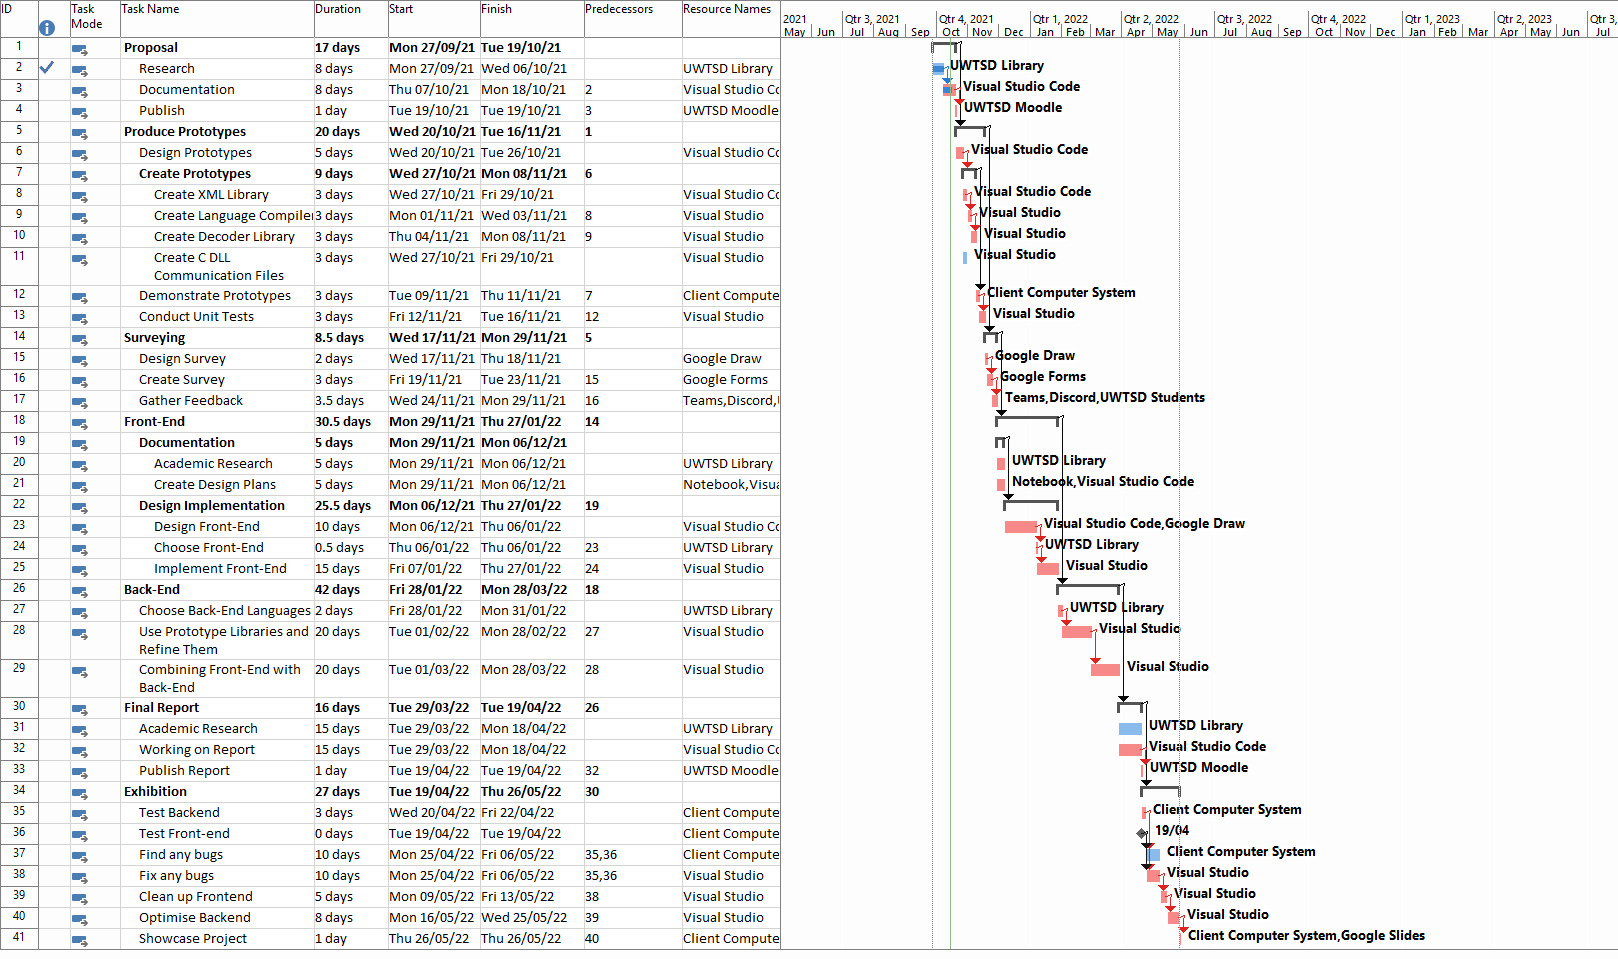
\includegraphics[height=.60\textheight, width=1.30\textwidth]{Figures/VisualPro.jpg}
            \caption{VisualPro Gantt Chart}
          \end{figure}
      \end{landscape}
      %SUBSECTION END

      %SUBSECTION LANDSCAPE
      \begin{landscape}
        \thispagestyle{fancylandscape}
        \subsection{Mindmap - Ideas}
        This mindmap demonstrates the process and current experience, which helped get the idea for the final project.
        \begin{figure}[h]
          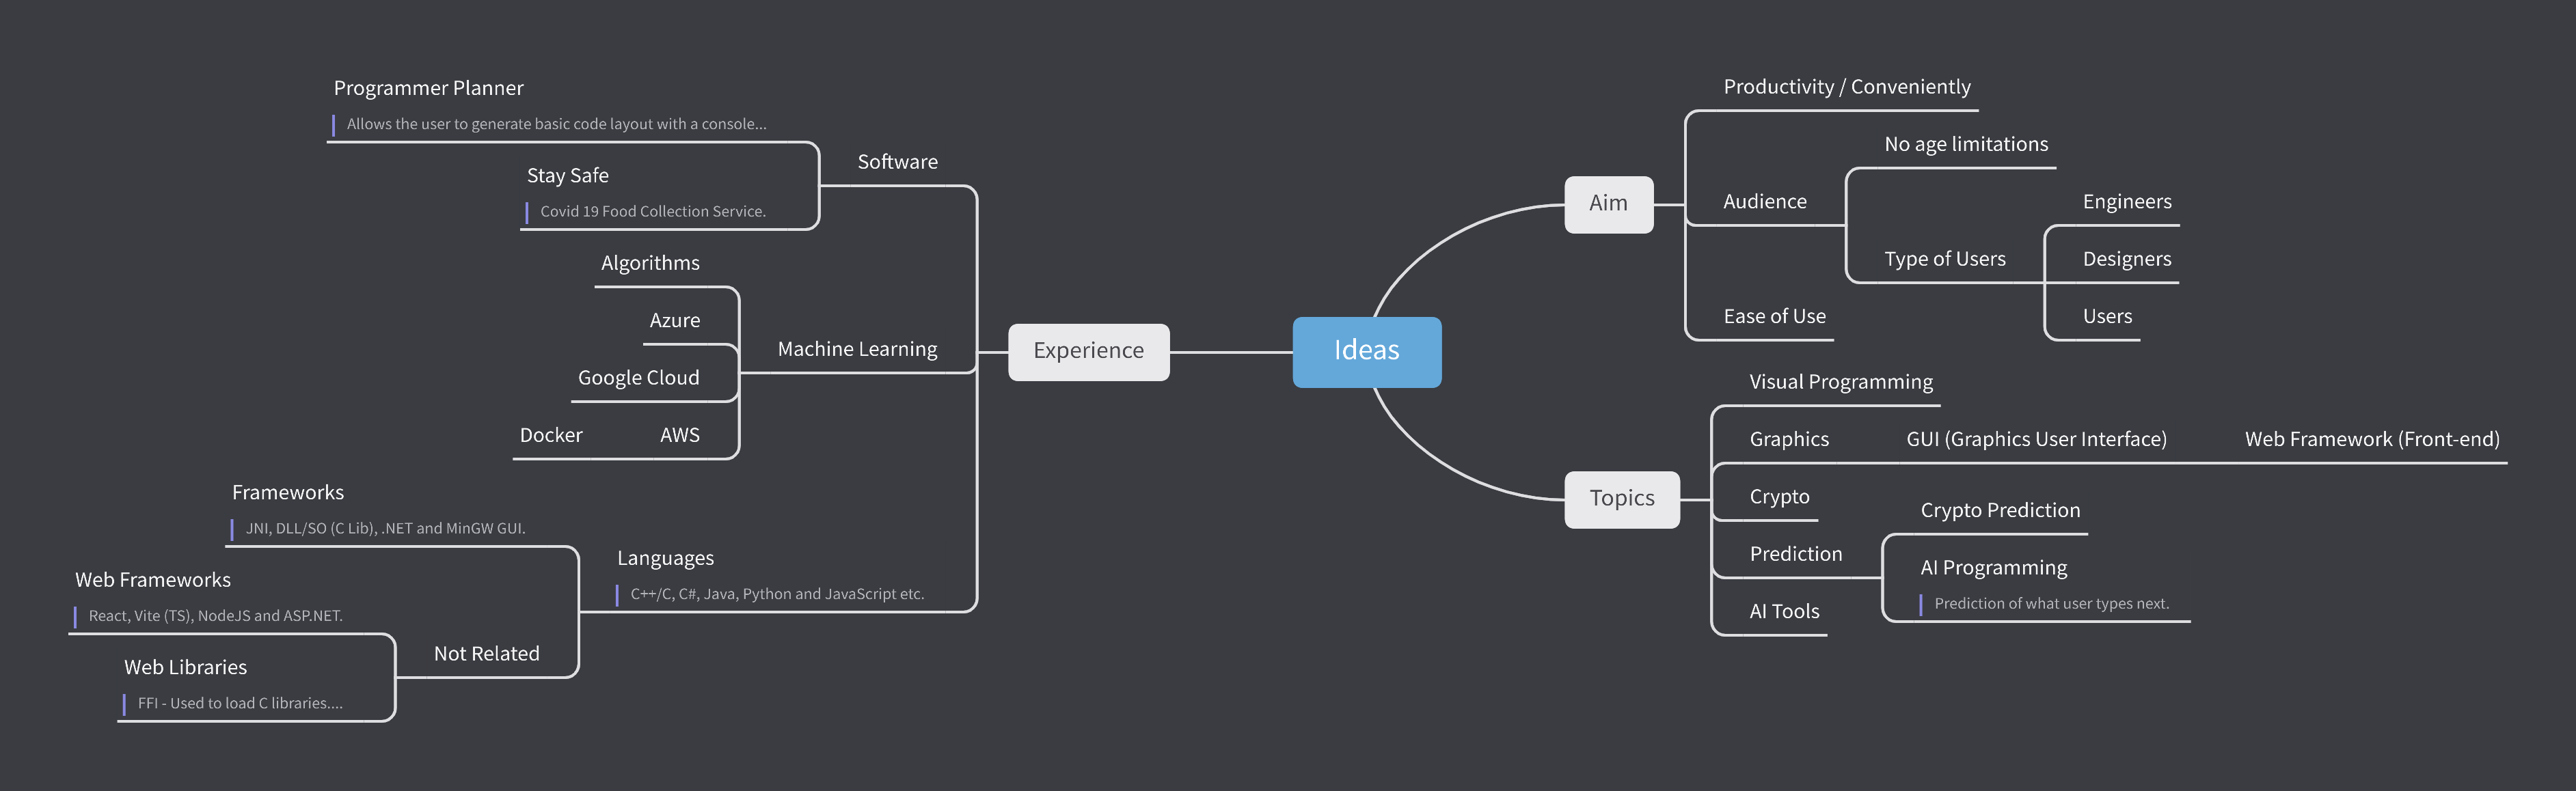
\includegraphics[height=.83\textheight, width=1.30\textwidth]{Figures/mindmap-ideas.png}
          \caption{VisualPro Ideas Mindmap}
        \end{figure}
      \end{landscape}
      %SUBSECTION END

      %SUBSECTION LANDSCAPE
      \begin{landscape}
        \thispagestyle{fancylandscape}
        \subsection{Mindmap - VisualPro}
        This mindmap displays existing and future libraries or problems within the final project that may prove resourceful within the development of VisualPro.
        \begin{figure}[h]
          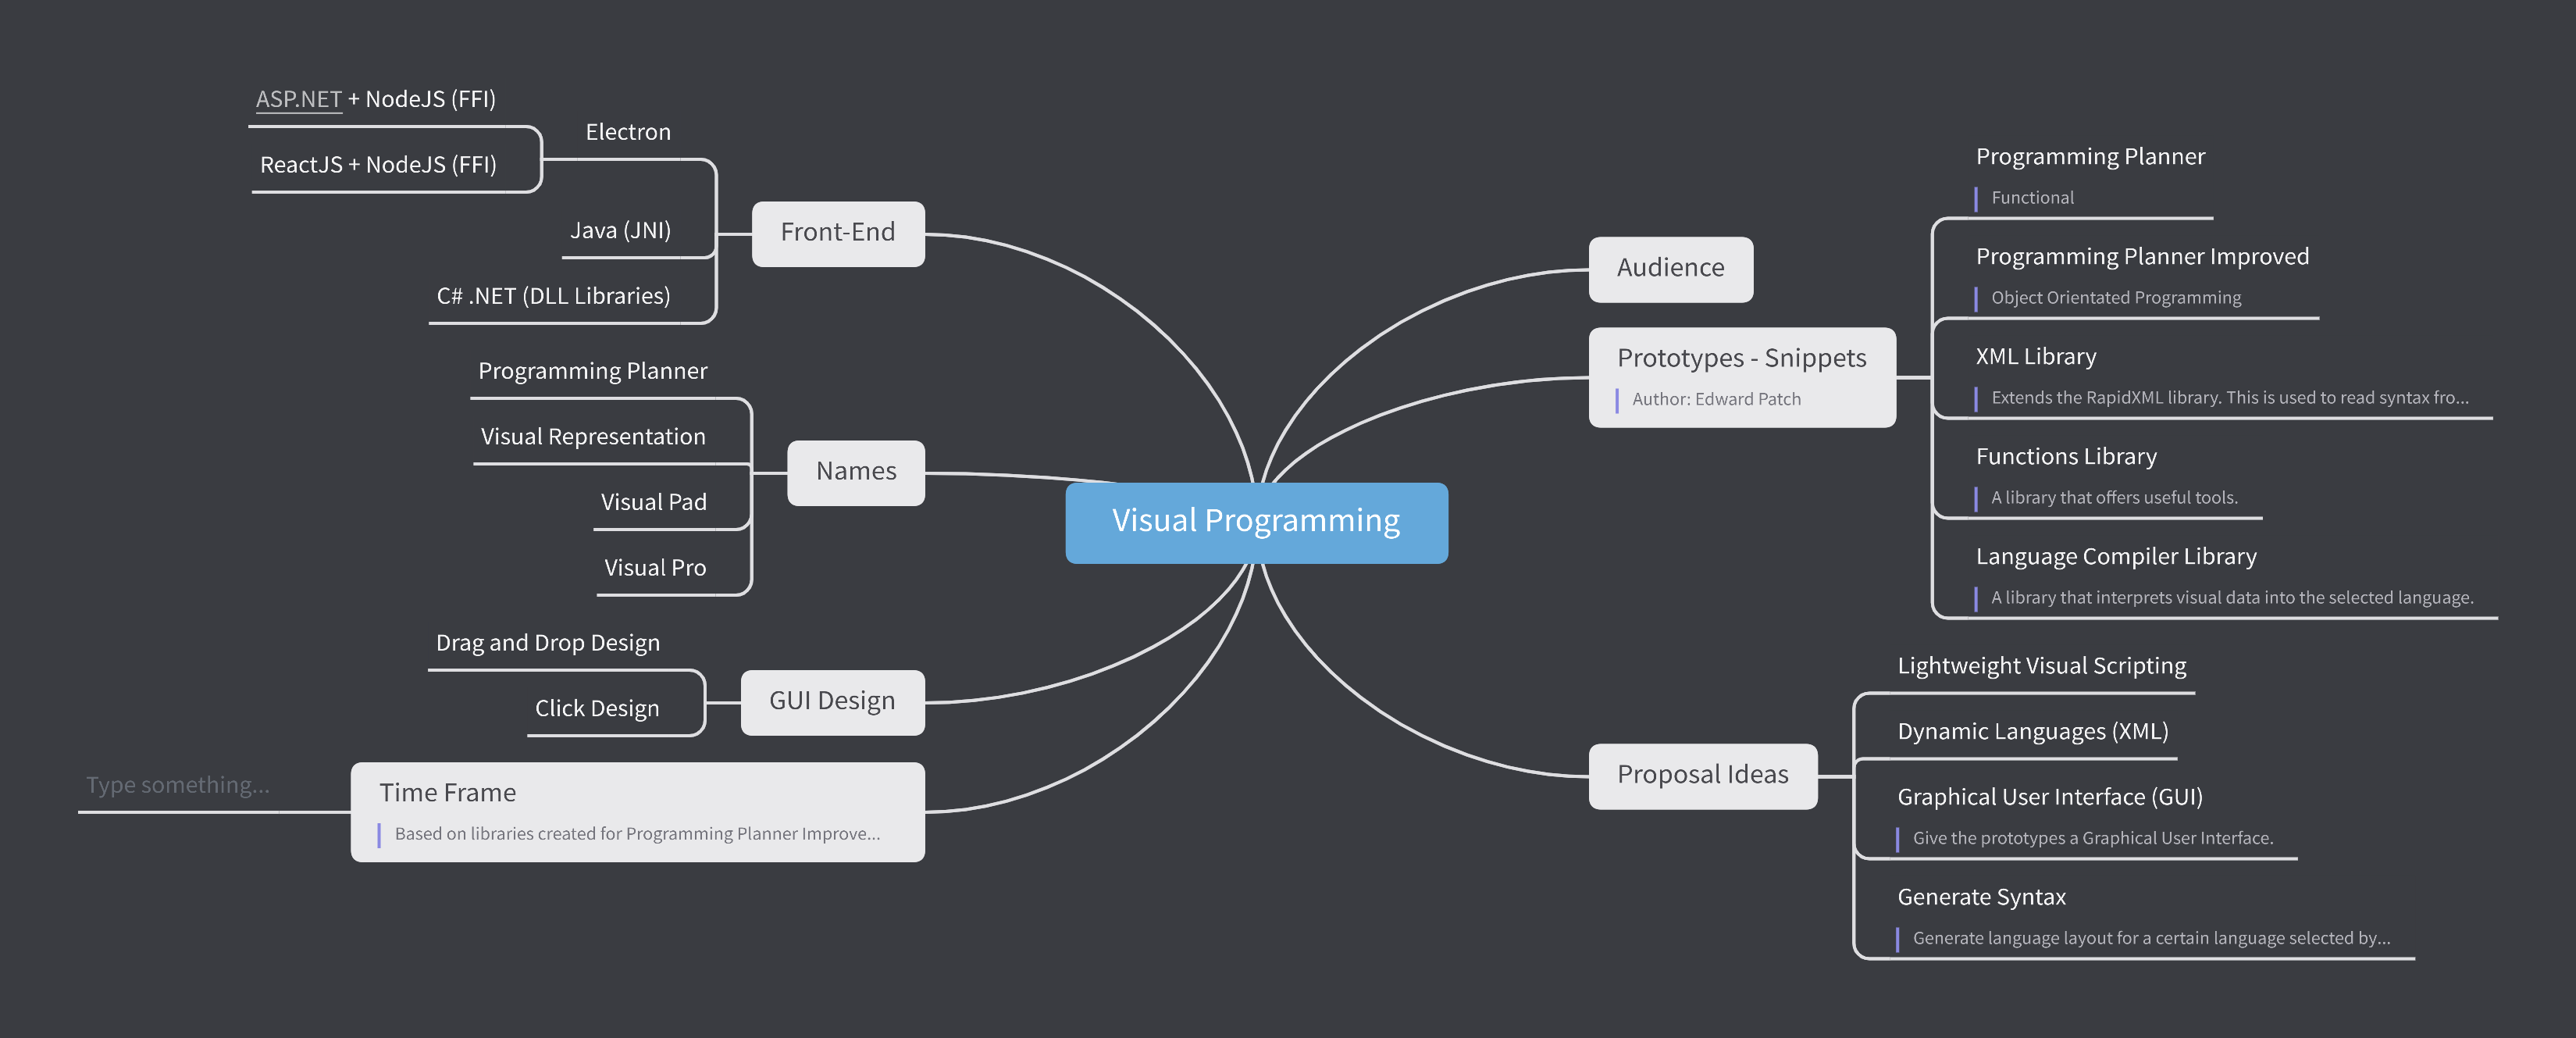
\includegraphics[height=.83\textheight, width=1.30\textwidth]{Figures/mindmap-vp.png}
          \caption{VisualPro Mindmap}
        \end{figure}
      \end{landscape}
      %SUBSECTION END

    \section{Terminology}
      List of terminologies used in this document:-
      \begin{itemize}
        \item GUI - Graphical User Interface.
        \item XML - Extensible Markup Language.
        \item DLL - Dynamic-Link Library.
        \item MMW - Multimedia Workshop.
      \end{itemize}
  
    \section{Appendices}

  %\nocite{*}
	\renewcommand\refname{\section{Reference List}}
	\small{\bibliographystyle{IEEEtran}
    \bibliography{ref}}
\end{document}